We consider software transactional memory (STM) concurrency control for multicore real-time software, and present a novel contention manager (CM) for resolving transactional conflicts, called Priority contention manager with Negative values and First access (PNF). We upper bound transactional retries and response times under PNF, when used with G-EDF and  G-RMA schedulers. We identify the conditions under which PNF outperforms previous real-time STM CMs and lock-free synchronization. Our work reveals that G-EDF/PNF and G-RMA/PNF have shorter or comparable retry costs and response times than other synchronization techniques.

\section{ECM and RCM: Overview and Limitations\label{probelm description}}

ECM and RCM~\cite{stmconcurrencycontrol:emsoft11} use dynamic and fixed priorities, respectively, to resolve transactional conflicts. ECM is used with the G-EDF scheduler, and allows the transaction whose job has the earliest absolute deadline to commit first~\cite{6045438}. RCM is used with the G-RMA scheduler, and allows the transaction whose job has the shortest relative deadline to commit first.

%%BR: I wonder whether it would be useful for Systor reviewers to know about the retry upper bounds of ECM and RCM. You can simply state those theorems here: "Retry costs under ECM is bounded in~\cite{stmconcurrencycontrol:emsoft11} as follows:"
%%BR: Now state the theorem with a citation: "Theorem 1 (from [])..."
%%BR: (no need to provide the proof). Also, your notations also carry over and have been defined in this paper.
%%BR: Now repeat for RCM's bound. 

As mentioned before, \cite{stmconcurrencycontrol:emsoft11} assumes that each transaction accesses only one object. This assumption simplifies the retry cost (Claims 2 and 3 in~\cite{stmconcurrencycontrol:emsoft11}) and response time analysis (Sections 4 and 5 in~\cite{stmconcurrencycontrol:emsoft11}). Besides, it enables a one-to-one comparison with retry-loop lock-free synchronization in~\cite{key-5}. With multiple objects per transaction, \cite{stmconcurrencycontrol:emsoft11} will introduce transitive retry, which we illustrate with an example.


\textbf{Example 1.} Consider three atomic sections $s_{1}^{x}$, $s_{2}^{y}$, 
and $s_{3}^{z}$ belonging to jobs $\tau_{1}^{x}$,$\tau_{2}^{y}$, 
and $\tau_{3}^{z}$, with priorities $p_{3}^{z}>p_{2}^{y}>p_{1}^{x}$, respectively. 
Assume that $s_{1}^{x}$ and $s_{2}^{y}$ share objects, $s_{2}^{y}$ and $s_{3}^{z}$
share objects. $s_{1}^{x}$ and $s_{3}^{z}$ do not share objects.
$s_{3}^{z}$ can cause $s_{2}^{y}$ to retry, which in turn will cause $s_{1}^{x}$ to retry. 
This means that $s_{1}^{x}$ may retry transitively
because of $s_{3}^{z}$, which will increase the retry cost of $s_{1}^{x}$.

Assume another atomic section $s_4^f$ is introduced. Priority of $s_4^f$ is higher than priority of $s_3^z$. $s_4^f$ shares objects only with $s_3^z$. Thus, $s_4^f$ can make $s_3^z$ to retry, which in turn will make $s_2^y$ to retry, and finally, $s_1^x$ to retry. Thus, transitive retry will move from $s_{4}^{f}$ to $s_{1}^{x}$, increasing the retry cost of $s_{1}^{x}$. 
The situation gets worse as more tasks of higher priorities are added, where each task
shares objects with its immediate lower priority task. $\tau_{3}^{z}$
may have atomic sections that share objects with $\tau_{1}^{x}$,
but this will not prevent the effect of transitive retry due to $s_{1}^{x}$.

\begin{mydef}
\textbf{Transitive Retry:} A transaction $s_{i}^{k}$ suffers from
transitive retry when it conflicts with a higher priority transaction
$s_{j}^{l}$, which in turn conflicts with a higher priority transaction
$s_{z}^{h}$, but $s_{i}^{k}$ does not conflict with $s_{z}^{h}$.
Still, when $s_{j}^{l}$ retries due to $s_{z}^{h}$, $s_{i}^{k}$
also retries due to $s_{j}^{l}$. Thus, the effect of the higher priority
transaction $s_{z}^{h}$ is transitively moved to the lower priority
transaction $s_{i}^{k}$, even when they do not conflict on common objects.
\end{mydef}

\begin{clm}\label{ecm-rcm-transitive-retry}
ECM and RCM suffer from transitive retry for multi-object transactions.
\end{clm}
\begin{proof}
ECM and RCM depend on priorities to resolve conflicts between transactions. Thus, lower priority transaction must always be aborted for a conflicting higher priority transaction. Claim follows. 
\end{proof}

Therefore, the analysis in~\cite{stmconcurrencycontrol:emsoft11} must extend the set of objects that can cause an atomic section of a lower priority job to retry.  This can be done by initializing the set of conflicting objects, $\gamma_i$, to all objects accessed by all transactions of $\tau_i$. We then cycle through all transactions belonging to all other higher priority tasks. Each transaction $s_j^l$ that accesses at least one of the objects in $\gamma_i$ adds all other objects accessed by $s_j^l$ to $\gamma_i$. The loop over all higher priority tasks is repeated, each time with the new $\gamma_i$, until there are no more transactions accessing any object in $\gamma_i$\footnote{However, note that, this solution may over-extend the set of conflicting objects, and may even contain all objects accessed by all tasks.}.

In addition to the \emph{transitive retry} problem, retrying higher priority transactions can prevent lower priority tasks from running. This happens when all processors are busy with higher priority jobs. When a transaction retries, the processor time is wasted. Thus, it would be better to give the processor to some other task.


Essentially, what we present is a new contention manager that avoids the effect of transitive retry. We call it, Priority contention manager with Negative values and First access (or P-N-F). P-N-F also tries to enhance processor utilization. This is done by allocating processors to jobs with non-retrying transactions. P-N-F is described in detail in Section \ref{P-N-F}.

\section{The P-N-F Contention Manager\label{P-N-F}}

\begin{algorithm}
\footnotesize{
\LinesNumbered
\KwData{
\textit{Executing Transaction:} is one that cannot be aborted by any other transaction, nor preempted by a higher priority task\;
\textit{$m$-set:} $m$-length set that contains only non-conflicting executing transactions\;
\textit{$n$-set:} $n$-length set that contains retrying transactions for $n$ tasks in non-increasing order of priority\;
\textit{n(z):} transaction at index $z$ of the $n$-set\;
$s_i^k$: a newly released transaction\;
$s_j^l$: one of the executing transactions\;
}
\KwResult{atomic sections that will commit}
\eIf{$s_i^k$ does not conflict with any executing transaction\label{s_i^k true}}
{
Assign $s_i^k$ as an executing transaction\;
Add $s_i^k$ to the $m$-set\;
Select $s_i^k$ to commit
}
{
Add $s_i^k$ to the $n$-set according to its priority\label{move to n}\;
Assign temporary priority -1 to the job that owns $s_i^k$ \label{priority to -1}\;
Select transaction(s) conflicting with $s_i^k$ for commit\label{s_i^k commit}\;
}
\If{$s_j^l$ commits\label{s_j^l commits}}
{
	\For{z=1 to size of n-set\label{traverse n-set}}
	{
		\If{n(z) does not conflict with any executing transaction\label{n(z) no conflict}}
		{
			\If{processor available\label{processor available}}
			{
				Restore priority of task owning n(z)\;
				Assign n(z) as executing transaction\;
				Add n(z) to m-set\;
				Select n(z) for commit\;
			}
		}
		move to the next n(z)\;
	}
}
}
\caption{P-N-F Algorithm} \label{P-N-F-algorithm}
\end{algorithm}

Algorithm \ref{P-N-F-algorithm} describes P-N-F. It
manages two sets. The first is the $m$-set, which contains at most $m$ non-conflicting
transactions, where $m$ is the number of processors, as
there cannot be more than $m$ executing transactions (or generally,
$m$ executing jobs) at the same time. When a transaction is entered
in the $m$-set, it executes non-preemptively and no other transaction
can abort it. A transaction in the $m$-set is called an \emph{executing
transaction}. 
This means that, when a transaction is executing before
the arrival of higher priority conflicting transactions, then the
one that started executing first will be committed (Step~\ref{s_i^k commit}) (hence the word ``First'' in the algorithm's name). 

The second set is the $n$-set, which holds the transactions
that are retrying because of a conflict with one or more of the executing
transactions (Step~\ref{move to n}), where $n$ stands for
the number of tasks in the system. It also holds transactions that
cannot currently execute, because processors are busy, either due to processing \emph{executing transactions}
and/or higher priority jobs. Any transaction in the $n$-set is assigned a temporal
priority of -1 (Step~\ref{priority to -1}) (hence the word 
``Negative'' in the algorithm's name). A negative priority
is considered smaller than any normal priority, and a transaction
continues to hold this negative priority until it is moved to the $m$-set, where it is restored its normal priority.


A job holding a transaction in the $n$-set can be preempted by any other job with normal priority, even if that normal priority job does not have transactions conflicting with the preempted job. Hence, this set is of length $n$, as there can be at most $n$ jobs in the system at the
same time. Transactions in the $n$-set whose jobs have been preempted are called \emph{preempted transactions}.
%%%
%%%
%BR: From here on, there is no need to italicize  \emph{preempted transactions} and \emph{executing transactions}. (First time is okay.) Remove all such emphasis from here. 
The $n$-set list keeps track of \emph{preempted transactions}, because
as it will be shown, \emph{preempted transactions} are examined when any of the
\emph{executing transaction} commits. Then, one or more transactions are selected from the $m$-set to be \emph{executing transactions}. If a \emph{preempted transaction} is selected as an \emph{executing transaction}, then the task that owns the \emph{preempted transaction} regains its priority. Thus, an aborted transaction can preempt the job which previously preempted it when the transaction was in the $n$-set.

When a new transaction is released, and it does not conflict with
any of the \emph{executing transactions} (Step~\ref{s_i^k true}), then
it will allocate a slot in the $m$-set and becomes an
\emph{executing transaction} itself. When this transaction is released (which means that its containing task is already allocated to a processor), it will be able to access a processor immediately. 
This new transaction may have a conflict with any of the transactions in the $n$-set. However, since transactions in the $n$-set have priorities of -1, they cannot prevent this new transaction from executing if it does not conflict with any of the \emph{executing transactions}.

When one of the \emph{executing transactions} commits (Step~\ref{s_j^l commits}), it is time to select one of the $n$-set transactions to
commit. The $n$-set is traversed from the highest priority
transaction to the lowest priority (where priority here refers to the
original priority of the transactions, and not -1) (Step~\ref{traverse n-set}).

If an examined transaction in the $n$-set, $s_{h}^{b}$,
does not conflict with any \emph{executing transaction} (Step~\ref{n(z) no conflict}),
and there is an available processor for it (Step~\ref{processor available})
(where ``available'' means either an idle processor, or one that
is executing a job of lower priority than $s_{h}^{b}$),
then $s_{h}^{b}$ is moved from the $n$-set to the
$m$-set, as an \emph{executing transaction} and restored its original priority. 

If $s_{h}^{b}$ is added to the $m$-set, the new $m$-set is used to compare with other transactions in the $n$-set with lower priority than $s_{h}^{b}$. 
Hence, if one of the transactions in the $n$-set, $s_{d}^{g}$, is of
lower priority than $s_{h}^{b}$ and conflicts with $s_{h}^{b}$,
it will remain in the $n$-set. 

The choice of the new transaction
from the $n$-set depends on the original priority of transactions (hence the word  ``PCM'' in the name of the algorithm). Thus, the algorithm
avoids interrupting an already executing transaction to reduce its
retry cost. In the meanwhile, it tries to avoid delaying the highest priority
transaction in the $n$-set when it is time to select a new
one to commit, even if the highest priority transaction arrives after
other lower priority transactions in the $n$-set.

%%BR: How about a subsection here called "Illustrative Example", where you show how P-N-F works for an example task set? Use a small task set with 3-4 tasks, etc. That will significantly help the reviewers. 

\subsection{Properties\label{pnf properties sec}}

\begin{clm}\label{P-N-F-transitive-retry}
Transactions scheduled under P-N-F do not suffer from transitive
retry.
\end{clm}
\begin{proof}
The proof is by contradiction. Assume that a transaction $s_{i}^{k}$
is retrying because of a higher priority transaction $s_{j}^{l}$, which
in turn is retrying because of another higher priority transaction
$s_{z}^{h}$. Assume that $s_{i}^{k}$ and $s_{z}^{h}$ do not conflict, yet,
$s_{i}^{k}$ is transitively retrying because of $s_{z}^{h}$. 
Note that $s_{z}^{h}$ and $s_{j}^{l}$ cannot exit together in
the $m$-set as they have common objects. But they both can
exist in the $n$-set, as they both can conflict with other \emph{executing
transactions}. We have three cases:

\textit{Case 1:} Assume that $s_{z}^{h}$ is an \emph{executing transaction}. This means that $s_{j}^{l}$ is in the $n$-set. When $s_{i}^{k}$ arrives, by the definition of P-N-F, it will be compared with the $m$-set, which contains $s_{z}^{h}$. Now, it will be found that $s_{i}^{k}$ does not conflict with $s_{z}^{h}$. Also, by the definition of P-N-F, $s_{i}^{k}$ is not compared with transactions in the $n$-set. When it newly arrives, priorities of $n$-set transactions are lower than any normal priority. Therefore, as $s_{i}^{k}$ does not conflict with any other executing
transaction, it joins the $m$-set and becomes an \emph{executing
transaction}. This contradicts the assumption that $s_{i}^{k}$
is transitively retrying because of $s_{z}^{h}$.



\textit{Case 2:} Assume that $s_{z}^{h}$ is in the $n$-set, while $s_{j}^{l}$
is an executing transaction. When $s_{i}^{k}$ arrives, it will conflict
with $s_{j}^{l}$ and joins the $n$-set. Now, $s_{i}^{k}$
retries due to $s_{j}^{l}$, and not $s_{z}^{h}$. When $s_{j}^{l}$ commits,
the $n$-set is traversed from the highest priority transaction
to the lowest one: if $s_{z}^{h}$ does not conflict with any other
executing transaction and there are available processors, $s_{z}^{h}$
becomes an executing transaction. When $s_{i}^{k}$ is compared with 
the $m$-set, it is found that it does not conflict with $s_{z}^{h}$. Additionally, if it also does not conflict with any other executing transaction and there are available processors, then $s_{i}^{k}$ becomes an executing
transaction. This means that $s_{i}^{k}$ and $s_{z}^{h}$ are executing
concurrently, which violates the assumption of transitive retry.

\textit{Case 3:} Assume that $s_{z}^{h}$ and $s_{j}^{l}$ both exist in the $n$-set.
When $s_{i}^{k}$ arrives, it is compared with the $m$-set. If $s_{i}^{k}$ does not conflict with any executing transactions and there are available processors, then $s_{i}^{k}$ becomes an executing transaction. 
Even though $s_{i}^{k}$ has common objects with $s_{j}^{l}$, $s_{i}^{k}$ is not compared with $s_{j}^{l}$, which is in the $n$-set. If $s_{i}^{k}$ joins the $n$-set, it is because, it conflicts with one or more executing transactions, not because of $s_{z}^{h}$, which violates the transitive retry assumption.
If the three transactions $s_i^k$, $s_j^l$ and $s_z^h$ exist in the $n$-set, and  $s_{z}^{h}$ is chosen as a new executing transaction, then $s_{j}^{l}$ remains in the $n$-set. This leads to
Case 1. If $s_{j}^{l}$ is chosen, because $s_{z}^{h}$ conflicts
with another executing transaction and $s_{j}^{l}$ does not, then
this leads to Case 2. Claim follows.
%
\end{proof}


\begin{clm}\label{first-access}
The \emph{first access} property of P-N-F is important
to avoid increased retry cost of transactions suffering from transitive
retry.
%%BR: This is badly worded! A claim should be quantitative or at least stating that something won't happen (e.g., "X protocol prevents deadlocks"). Saying that something is important as a claim doesn't make any sense. Reword (e.g., "The \emph{first access} property of P-N-F bounds the transitive retry cost of transactions.")
\end{clm}
\begin{proof}
The proof is by contradiction. Assume that the retry cost of transactions
in the absence of the first access property is the same as when first access  exists. Now, assume that P-N-F is devoid of the first access property.  This means that executing transactions can be aborted. 

Assume three transactions $s_{i}^{k}$, $s_{j}^{l}$, and $s_{z}^{h}$, where $s_{z}^{h}$'s priority is higher than $s_{j}^{l}$'s priority, and $s_j^l$'s priority is higher than $s_{i}^{k}$'s priority. Assume that $s_{j}^{l}$ conflicts with both $s_{i}^{k}$ and $s_{z}^{h}$. 
$s_{i}^{k}$ and $s_{z}^{h}$ do not conflict together. If $s_{i}^{k}$
arrives while $s_{z}^{h}$ is an \emph{executing transaction} and $s_{j}^{l}$
exists in the $n$-set, then $s_{i}^{k}$ becomes an \emph{executing transaction} itself while $s_{j}^{l}$ is retrying. If $s_{i}^{k}$ did not commit at least when $s_{z}^{h}$ commits, then $s_{j}^{l}$ becomes an executing transaction. 
Due to the lack of the first access property, $s_{j}^{l}$ will cause $s_{i}^{k}$ to retry. So, the retry cost for $s_{i}^{k}$ will be $len(s_{z}^{h}+s_{j}^{l})$. This
retry cost for $s_{i}^{k}$ is the same if it had been transitively
retrying because of $s_{z}^{h}$. 
This contradicts the first
assumption. Claim follows.
\end{proof}

%%
%\begin{clm}
%P-N-F handles multi-object transactions better than ECM and RCM.
%\end{clm}
%\begin{proof}
%%BR: I suggest not stating this as a claim, as it is quite straightforward from the previous ones. 
From Claims \ref{P-N-F-transitive-retry} and \ref{first-access}, P-N-F does not increase the retry cost of multi-object transactions. However, this is not the case for ECM and RCM as shown by Claim~\ref{ecm-rcm-transitive-retry}. %Claim follows.
%\end{proof}

\begin{clm}\label{higher retry does not affect response}
Under P-N-F, any job $\tau_{i}^{x}$ is not affected by the retry cost in any other
job $\tau_{j}^{l}$.
\end{clm}
\begin{proof}
As explained in Section~\ref{P-N-F-algorithm}, P-N-F assigns a temporary priority of -1 to any job that includes a retrying transaction. So, retrying transactions have lower priority than any other normal priority.
When $\tau_{i}^{x}$ is released and $\tau_j^l$ has a retrying transaction, $\tau_i^x$ will have a higher priority
than $\tau_j^l$. Thus, $\tau_i^x$ can run on any available processor while $\tau_j^l$ is retrying one of its transactions. Claim follows.
\end{proof}


\section{Retry Cost under P-N-F\label{rc pnf sec}}

We now derive an upper bound on the retry cost of any job $\tau_i^x$ under P-N-F during an interval $L\le T_i$. Since all tasks are sporadic (i.e., each task $\tau_i$ has a minimum period $T_i$), $T_i$ is the maximum study interval for each task $\tau_i$.

\begin{clm}\label{two transactions retry cost P-N-F}
Assume two conflicting transactions $s_{i}^{k}$ and $s_{j}^{l}$.
Under P-N-F, the maximum retry cost suffered by $s_{i}^{k}$ due
to $s_{j}^{l}$ is $len(s_{j}^{l})$.
\end{clm}
\begin{proof}
By P-N-F's definition, $s_{i}^{k}$ cannot have started before
$s_{j}^{l}$. Otherwise, $s_i^k$ would have been an \emph{executing transaction} and $s_{j}^{l}$ cannot abort it. So, the earliest release time for $s_{i}^{k}$ would have been just after $s_{j}^{l}$ starts execution. Then, $s_i^k$ would have to wait until $s_{j}^{l}$
commits. Claim follows.
\end{proof}

\begin{clm}
The retry cost for any job $\tau_{i}^{x}$ due to conflicts between its transactions and transactions of other jobs under P-N-F during an interval $L\le T_{i}$ is upper bounded by:
\begin{equation}
RC(L)\le\sum_{\tau_{j}\in\gamma_{i}}\left(\sum_{\theta\in\theta_{i}}\left(\left(\left\lceil \frac{L}{T_{j}}\right\rceil +1\right)\sum_{\bar{\forall s_{j}^{l}(\theta)}}len\left(\bar{s_{j}^{l}(\theta)}\right)\right)\right)\label{rc-P-N-F}
\end{equation}
where $\bar{s_{j}^{l}(\theta)}$ is the same as $s_{j}^{l}(\theta)$ except for the following difference:
 if $\bar{s_{j}^{l}}$ accesses multiple objects in $\theta_{i}$,
then $\bar{s_{j}^{l}}$ is included only once in the last summation (i.e., $\bar{s_j^l}$ is not repeated for each shared object with $s_i^k$).
\end{clm}
\begin{proof}
Consider a transaction $s_{i}^{k}$ belonging to job $\tau_{i}^{x}$. Under P-N-F, higher priority transactions than $s_i^k$ can become \emph{executing transactions} before $s_i^k$. A lower priority transaction $s_v^f$ can also become an \emph{executing transaction} before $s_i^k$. This happens when $s_i^k$ conflicts with any \emph{executing transaction} while $s_v^f$ does not. The worst case scenario for $s_{i}^{k}$ occurs when $s_i^k$ has to wait in the $n$-set, while all other conflicting transactions with $s_i^k$ are chosen to be \emph{executing transactions}. 
Let $\bar{s_j^l}$ accesses multiple objects in $\theta_i$. If $\bar{s_j^l}$ is an \emph{executing transaction}, then $\bar{s_j^l}$ will not repeat itself for each object it accesses. Besides, $\bar{s_j^l}$ will finish before $s_i^k$ starts execution. Consequently, $\bar{s_j^l}$ will not conflict with $s_i^{k+1}$. This means that an \emph{executing transaction} can force no more than one transaction in a given job to retry. This is why $\bar{s_j^l}$ is included only once in~(\ref{rc-P-N-F}) for all shared objects with $s_i^k$.

The maximum number of jobs of any task $\tau_{j}$ that can interfere with $\tau_{i}^{x}$ during interval $L$ is $\left\lceil \frac{L}{T_{j}}\right\rceil +1$. From  the previous observations and Claim~\ref{two transactions retry cost P-N-F}, Claim follows.
\end{proof}

\begin{clm}\label{delay}
The delay time for a 
%%BR: "delay time" is somewhat awkward. How about "blocking time"? Use it consistently throughout the paper. 
job $\tau_{i}^{x}$ due to lower priority jobs,
during an interval $L\le T_{i}$, is upper bounded by:
\begin{equation}
D(\tau_{i}^{x})\le\left\lfloor \frac{1}{m}\sum_{\forall\bar{\tau_{j}^{l}}}\left(\left(\left\lceil \frac{L}{T_{j}}\right\rceil +1\right)\sum_{\forall\ddot{s_{j}^{h}}}len\left(\ddot{s_{j}^{h}}\right)\right)\right\rfloor \label{P-N-F-delay}
\end{equation}
where $D(\tau_{i}^{x})$ is the delay time 
%%BR: "blocking time"? 
suffered by $\tau_{i}^{x}$
due to lower priority jobs. $\bar{\tau_{j}^{l}}=\{\tau_{j}^{l}:p_{j}^{l}<p_{i}^{x}\}$
and $\ddot{s_{j}^{h}}=\{s_{j}^{h}:s_{j}^{h}\, does\, not\, conflict\, with\, any\, s_{i}^{k}\}$.
During this delay time, 
%%BR: "blocking time"? 
all processors are unavailable for $\tau_{i}^{x}$.
\end{clm}
\begin{proof}
Under P-N-F, \emph{executing transactions} are non-preemptive. So, lower priority \emph{executing transactions} can delay a higher priority job $\tau_i^x$ if no other processors are available. Lower priority executing transactions can be conflicting or non-conflicting with any transaction in $\tau_{i}^{x}$. They also can exist when $\tau_i^x$ is newly released, or after that. So, we have the following cases:

\emph{Lower priority conflicting transactions after $\tau_i^x$ is released:} This case is already covered by the retry cost in~(\ref{rc-P-N-F}).

\emph{Lower priority conflicting transactions when $\tau_i^x$ is newly released:} Each lower priority conflicting transaction $s_j^h$ will delay $\tau_i^x$ for $len(s_j^h)$. The effect of $s_j^h$ is already covered by~(\ref{rc-P-N-F}). Besides,~(\ref{rc-P-N-F}) does not divide the retry cost by $m$ as done in~(\ref{P-N-F-delay}). Thus, the worst case scenario requires inclusion of $s_j^h$ in~(\ref{rc-P-N-F}), and not in~(\ref{P-N-F-delay}).

\emph{Lower priority non-conflicting transactions when $\tau_i^x$ is newly released:} $\tau_i^x$ is delayed if there are no available processors for it. Otherwise, $\tau_i^x$ can run in parallel with these non-conflicting lower priority transactions. Each lower priority non-conflicting transaction $\ddot{s_j^h}$ will delay $\tau_i^x$ for $len(\ddot{s_j^h})$.

\emph{Lower priority non-conflicting transactions after $\tau_i^x$ is released:} This situation can happen if $\tau_i^x$ is retrying one of its transactions $s_i^k$. So, $\tau_i^x$ is assigned a priority of -1. $\tau_i^x$ can be preempted by any other job. When $s_i^k$ is checked again to be an \emph{executing transaction}, all processors may be busy with lower priority non-conflicting transaction and/or higher priority jobs. Otherwise, $\tau_i^x$ can run in parallel with these lower priority non-conflicting transactions. The effect of higher priority jobs is included by Claims~\ref{response time ecm P-N-F}.
%,\ref{response rcm P-N-F}. 
%%BR: is there a need to cite the section? 
Each lower priority non-conflicting transaction $\ddot{s_j^h}$ will delay $\tau_i^x$ for $len(\ddot{s_j^h})$.

From the previous cases, lower priority non-conflicting transactions act as if they were higher priority jobs interfering with $\tau_{i}^{x}$. So, the delay time can be calculated by the interference workload given by Theorem 1 in \cite{key-2}. Claim follows.
\end{proof}


\begin{clm}\label{response time ecm P-N-F}
Assume that P-N-F is used with the G-EDF scheduler. The response
time of a job $\tau_{i}^{x}$, during an interval $L\le T_{i}$, is
upper bounded by:
\begin{equation}
R_{i}^{up}=c_{i}+RC(L)+D_{edf}(\tau_{i}^{x})+\left\lfloor \frac{1}{m}\sum_{\forall j\ne i}W_{ij}(R_{i}^{up})\right\rfloor 
\end{equation}
where $RC(L)$ is calculated by (\ref{rc-P-N-F}). $D_{edf}(\tau_{i}^{x})$
is the same as $D(\tau_{i}^{x})$ defined in~(\ref{P-N-F-delay}). However, for G-EDF systems. $D_{edf}(\tau_i^x)$ is calculated as:
\begin{equation}
D_{edf}(\tau_{i}^{x})\le\left\lfloor \frac{1}{m}\sum_{\forall\bar{\tau_{j}^{l}}}\begin{cases}
0 & ,L\le T_{i}-T_{j}\\
\sum_{\forall\ddot{s_{j}^{h}}}len\left(\ddot{s_{j}^{h}}\right) & ,L>T_{i}-T_{j}
\end{cases}\right\rfloor \label{d-edf}
\end{equation}
and $W_{ij}(R_{i}^{up})$ is calculated by (3) in~\cite{stmconcurrencycontrol:emsoft11}.
\end{clm}
%%%%
%%%%%%%%%%
%%%%%%%%%%%
\begin{proof}
Response time for $\tau_{i}^{x}$ is calculated by (3) in~\cite{stmconcurrencycontrol:emsoft11} with the addition of delay time 
%%BR: blocking time?
defined by Claim \ref{delay}. G-EDF uses absolute deadlines for scheduling. This defines which jobs of the same task can be of lower priority than $\tau_{i}^{x}$, and which will not. Any instance $\tau_j^h$, released between $r_i^x - T_j$ and $d_i^x - T_j$, will be of higher priority than $\tau_i^x$. Before $r_i^x-T_j$, $\tau_j^h$ would have finished before $\tau_i^x$ is released. After $d_i^x-T_j$, $d_j^h$ would be greater than $d_i^x$. Thus, $\tau_j^h$ will be of lower priority than $\tau_i^x$. So, during $T_i$, there can be only one instance $\tau_j^h$ of $\tau_j$ with lower priority than $\tau_i^x$. $\tau_j^h$ is released between $d_i^x-T_j$ and $d_i^x$. Consequently, during $L<T_i-T_j$, no existing instance of $\tau_j$ is of lower  priority than $\tau_i^x$. Hence, 0 is used in the first case of~(\ref{d-edf}). But if $L>T_i-T_j$, there can be only one instance $\tau_j^h$ of $\tau_j$ with lower priority than $\tau_i^x$. Hence, $\left\lceil\frac{L}{T_i}\right\rceil+1$ in~(\ref{P-N-F-delay}) is replaced with 1 in the second case in~(\ref{d-edf}). Claim follows.
\end{proof}


\begin{clm}\label{response rcm P-N-F}
Assume that P-N-F is used with the G-RMA scheduler. Response
time of job $\tau_{i}^{x}$ during an interval $L\le T_{i}$ is upper
bounded by: 
\begin{equation}
R_{i}^{up}=c_{i}+RC(L)+D(\tau_{i}^{x})+\left\lfloor \frac{1}{m}\sum_{\forall j\ne i,p_j>p_i}W_{ij}(R_{i}^{up})\right\rfloor 
\end{equation}
where $RC(L)$ is calculated by (\ref{rc-P-N-F}), $D(\tau_{i}^{x})$
is calculated by (\ref{P-N-F-delay}), and $W_{ij}(R_{i}^{up})$
is calculated by (2) in~\cite{stmconcurrencycontrol:emsoft11}.
\end{clm}
\begin{proof}
The proof is the same as for Claim \ref{response time ecm P-N-F}, 
except that G-RMA assigns static priorities for tasks. Hence, (\ref{P-N-F-delay}) can be used directly for calculating $D(\tau_{i}^{x})$ without modifications. Claim follows.
\end{proof}


\section{Comparison between P-N-F and Other Synchronization Techniques}
\label{sec:pnf-sched-comparison}

We now (formally) compare the schedulability of G-EDF (G-RMA) with P-N-F against other synchronization techniques including the ECM and RCM STM contention managers~\cite{stmconcurrencycontrol:emsoft11} and retry-loop lock-free synchronization~\cite{stmconcurrencycontrol:emsoft11,key-5}. 
Such a comparison will reveal when P-N-F outperforms  others. 
Toward this, we compare the total utilization under G-EDF (G-RMA)/P-N-F,  with that under the other synchronization methods.
Inflated execution time of each method, which is the sum of the worst-case execution time of the task and its retry cost, is used in the utilization calculation of each task.

By Claim~\ref{delay}, no processor is available for $\tau_i^x$ during the delay time. As each processor is busy with some other job than $\tau_i^x$, $D(\tau_i^x)$ is not added to the inflated execution time of $\tau_i^x$. Hence, $D(\tau_i^x)$ is not added to the utilization calculation of $\tau_i^x$.

Let $RC_{A}(T_{i})$ denote the retry cost of any $\tau_i^x$ using the synchronization method $A$ during $T_i$. Let $RC_{B}(T_{i})$ denote the  retry cost of any $\tau_i^x$ using synchronization method $B$ during $T_i$. Then, schedulability of $A$ is comparable to $B$ if:
\begin{eqnarray}
\sum_{\forall\tau_{i}}\frac{c_{i}+RC_{A}(T_{i})}{T_{i}} & \le & \sum_{\forall\tau_{i}}\frac{c_{i}+RC_{B}(T_{i})}{T_{i}}\nonumber \\
\therefore\sum_{\forall\tau_{i}}\frac{RC_{A}(T_{i})}{T_{i}} & \le & \sum_{\forall\tau_{i}}\frac{RC_{B}(T_{i})}{T_{i}}\label{utilization comparison}
\end{eqnarray}


As described in Section~\ref{probelm description}, the set of common objects needs to be extended under ECM and RCM. Toward this, we introduce a few additional notions. Let $\theta_i^{ex}$ be an extended set of distinct objects that contains all objects in $\theta_i$. Thus, $\theta_i^{ex}$ contains all objects  accessed by $\tau_i$. $\theta_i^{ex}$ can also contain other objects that can cause any transaction in $\tau_i$ to retry as explained in Section~\ref{probelm description}. Thus, $\theta_i^{ex}$ may contain objects not accessed by $\tau_i$. $\gamma_i^{ex}$ is an extended set of tasks that access any object in $\theta_i^{ex}$. Therefore, $\gamma_i^{ex}$ contains at least all tasks in $\gamma_i$.

%%

There are two sources of retry cost for any $\tau_i^x$ under ECM, RCM, and lock-free. First is due to conflict between $\tau_i^x$'s transactions and transactions of other jobs. This is denoted as $RC$. Second is due to the preemption of any transaction in $\tau_i^x$ due to the release of a higher priority job $\tau_j^h$. This is denoted as $RC_{re}$. Retry due to the release of higher priority jobs do not occur under P-N-F,
because \emph{executing transactions} are non-preemptive. It is up to the implementation  of the contention manager to safely avoid $RC_{re}$. Here, we assume that ECM and RCM do not avoid $RC_{re}$. Thus, we introduce $RC_{re}$ for ECM and RCM first  before comparing P-N-F with other synchronization techniques.


\begin{clm}\label{ecm rlease conflict}
Under ECM, the total retry cost suffered by all transactions in any $\tau_i^x$ during an interval $L\le T_i$ is upper bounded by:
\begin{equation}
RC_{to}(L)=RC(L)+RC_{re}(L)
\label{total rc ecm eq}
\end{equation}
%
where $RC(L)$ is the retry cost resulting from conflict between transactions in $\tau_i^x$ and transactions of other jobs. $RC(L)$ is calculated by (15) in~\cite{stmconcurrencycontrol:emsoft11} with replacing $\gamma_i$ and $\theta_i$ with $\gamma_i^{ex}$ and $\theta_i^{ex}$, respectively. $RC_{re}(L)$ is the retry cost resulting from the release of higher priority jobs, which preempt $\tau_i^x$. $RC_{re}(L)$ is given by:
\begin{equation}
RC_{re}(L)=\sum_{\forall \tau_{j}\in\zeta_{i}}\begin{cases}
\left\lceil \frac{L}{T_{j}}\right\rceil s_{i_{max}} & ,L\le T_{i}-T_{j}\\\\
\left\lfloor \frac{T_{i}}{T_{j}}\right\rfloor s_{i_{max}} & ,L>T_{i}-T_{j}
\end{cases}\label{eq6}
\end{equation}
%
where $\zeta_i=\{\tau_j:\left(\tau_j \ne \tau_i\right)\wedge \left(D_j < D_i \right)\}$.
\end{clm}
\begin{proof}
Two conditions must be satisfied for any $\tau_{j}^{l}$ to be able to preempt
$\tau_{i}^{x}$ under G-EDF: $r_{i}^{x}<r_{j}^{l}<d_{i}^{x}$,
and $d_{j}^{l}\le d_{i}^{x}$. Without the first condition, $\tau_{j}^{l}$
would have been already released before $\tau_{i}^{x}$. Thus, $\tau_j^l$ will
not preempt $\tau_i^x$. Without the second condition, $\tau_{j}^{l}$ will
be of lower priority than $\tau_{i}^{x}$ and will not preempt it.
If $D_{j} \ge D_{i}$, then there will be at most one instance $\tau_j^l$ with higher priority than $\tau_{i}^{x}$. $\tau_j^l$ must have been released at most at $r_i^x$, which violates the first condition. The other instance $\tau_j^{l+1}$ would have an absolute deadline greater than $d_i^x$. This violates the second condition. Hence, only tasks with shorter relative deadline than $D_{i}$ are going to be considered. These jobs are grouped in $\zeta_i$.

The total number of released instances of $\tau_{j}$ during any interval $L\le T_{i}$ is $\left\lceil \frac{L}{T_{i}}\right\rceil +1$. The ``carried-in" jobs (i.e., each job released before $r_i^x$ and has an absolute deadline before $d_i^x$~\cite{key-2}) are discarded as they violate the first condition. The ``carried-out" jobs (i.e., each job released after $r_i^x$ and has an absolute deadline after $d_i^x$~\cite{key-2}) are also discarded because they violate the second condition. Thus, the number of considered higher priority instances of $\tau_j$ during the interval $L\le T_i-T_j$ is $\left\lceil\frac{L}{T_j}\right\rceil$. The number of considered higher priority instances of $\tau_j$ during interval $L> T_i-T_j$ is $\left\lfloor\frac{T_i}{T_j}\right\rfloor$.

The worst $RC_{re}$ for $\tau_i^x$ occurs when $\tau_i^x$ is always interfered at the end of execution of its longest atomic section, $s_{i_{max}}$. $\tau_i^x$ will have to retry for $len(s_{i_{max}})$, as shown in Figure~\ref{fig8}. The total retry cost suffered by $\tau_i^x$ is the combination of $RC$ and $RC_{re}$. Claim follows.

\begin{figure}
\centering{}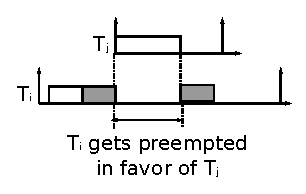
\includegraphics[scale=0.7]{figures/figure8}\caption{\label{fig8}Transactional retry due to release of higher priority
tasks}
\end{figure}
\end{proof}

\begin{clm}\label{rcm rlease conflict}
Under RCM, the total retry cost suffered by all transactions in any $\tau_i^x$ during an interval $L\le T_i$ is upper bounded by:
\begin{equation}
RC_{to}(L)=RC(L)+RC_{re}(L)
\label{total rc rcm eq}
\end{equation}
%
where $RC(L)$ and $RC_{re}(L)$ are defined in Claim~\ref{ecm rlease conflict}. $RC_{re}(L)$ is calculated by:
\begin{equation}
RC_{re}(L)=\sum_{\forall \tau_j \in \zeta_i^*}\left(\left\lceil\frac{L}{T_j}\right\rceil s_{i_{max}}\right)\label{eq21}
\end{equation}
%
where $\zeta_i^*=\{\tau_j:p_j > p_i \}$.
\end{clm}
\begin{proof}
The proof is the same as that for Claim~\ref{ecm rlease conflict}, except that G-RMA uses static priority. Thus, the carried-out jobs will be considered in the  interference with $\tau_i^x$. The carried-in jobs are still not considered because they are released before $r_i^x$. Claim follows.
\end{proof}
\begin{clm}\label{lock free release}
Consider retry-loop lock-free synchronization. Let $r_{i_{max}}$ be the maximum execution cost of a single iteration of any retry loop of $\tau_i$. $RC_{re}$ under G-EDF  with retry-loop lock-free synchronization is calculated by~(\ref{eq6}), where $s_{i_{max}}$ is replaced by $r_{i_{max}}$. $RC_{re}$ under G-RMA with retry-loop lock-free synchronization is calculated by~(\ref{eq21}), where $s_{i_{max}}$ is replaced by $r_{i_{max}}$.
\end{clm}
%
\begin{proof}
The interference pattern of higher priority jobs to lower priority jobs is the same in ECM and G-EDF with retry-loop lock-free synchronization. The pattern is also the same in RCM and G-RMA with retry-loop lock-free. Claim follows.
\end{proof}


\subsection{P-N-F versus ECM\label{pnf vs ecm sec}}

\begin{clm}\label{P-N-F ecf comaprison clm}
The schedulability of P-N-F with G-EDF tends to be
%%BR: "tends to be" is weak. Why don't you say "is"?
 better or equal to the schedulability  of ECM when conflicting atomic sections have equal lengths.
\end{clm}
\begin{proof}
Substitue $RC_{A}(T_{i})$ and $RC_{B}(T_{i})$ in (\ref{utilization comparison})
with (\ref{rc-P-N-F}) and (\ref{total rc ecm eq}), respectively. Let $\theta_{i}^{ex}=\theta_{i}+\theta_{i}^{*}$, where $\theta_{i}^{*}$
is the set of objects not accessed directly by $\tau_{i}$ but can
cause transactions in $\tau_{i}$ to retry due to transitive retry.
Let $\gamma_{i}^{ex}=\gamma_{i}+\gamma_{i}^{*}$, where $\gamma_{i}^{*}$
is the set of tasks that access objects in $\theta_{i}^{*}$.

Let:
%
\begin{comment}
\begin{eqnarray*}
g(\tau_{i}) & = & \left(\sum_{\forall\tau_{j}\in\gamma_{i}^{*}}\sum_{\theta\in\theta_{i}^{*}}\left(\left\lceil \frac{T_{i}}{T_{j}}\right\rceil \sum_{\forall\bar{s_{j}^{k}(\theta)}}len\left(\bar{s_{j}^{k}(\theta)}\\
& + & s_{max}^{*}(\theta)\right)\right)\right) + RC_{re}(T_{i})
\end{eqnarray*}
\end{comment}
\begin{eqnarray*}
g(\tau_{i}) & = & \Bigg(\sum_{\forall\tau_{j}\in\gamma_{i}^{*}}\sum_{\theta\in\theta_{i}^{*}}\Bigg(\left\lceil \frac{T_{i}}{T_{j}}\right\rceil \sum_{\forall\bar{s_{j}^{k}(\theta)}}len\Big(\bar{s_{j}^{k}(\theta)}\\
 & + & s_{max}^{*}(\theta)\Big)\Bigg)\Bigg)+RC_{re}(T_{i})
\end{eqnarray*}
%
where $RC_{re}$ is given by~(\ref{eq6}). Let:
%
\begin{equation*}
\eta_{1}(\tau_{i})=\sum_{\forall\tau_{j}\in\gamma_{i}}\sum_{\forall\theta\in\theta_{i}}\left(\sum_{\bar{\forall s_{j}^{k}(\theta)}}len\left(\bar{s_{j}^{k}(\theta)}\right)\right)
\end{equation*}
%
\begin{equation*}
\eta_{2}(\tau_{i})=\sum_{\forall\tau_{j}\in\gamma_{i}}\sum_{\forall\theta\in\theta_{i}}\left(\left\lceil \frac{T_{i}}{T_{j}}\right\rceil \sum_{\forall\bar{s_{j}^{k}(\theta)}}len\left(s_{max}^{j}(\theta)\right)\right)
\end{equation*}
%
and
%
\begin{equation*}
\eta_{3}(\tau_{i})=\sum_{\forall\tau_{j}\in\gamma_{i}}\sum_{\forall\theta\in\theta_{i}}\left(\left\lceil \frac{T_{i}}{T_{j}}\right\rceil \sum_{\bar{\forall s_{j}^{k}(\theta)}}len\left(\bar{s_{j}^{k}(\theta)}\right)\right)
\end{equation*}
%
By substitution of $g(\tau_{i})$, $\eta_1(\tau_i)$, and $\eta_2(\tau_i)$, and subtraction of $\sum_{\forall \tau_i} \frac{\eta_3(\tau_i)}{T_i}$ from both sides of (\ref{utilization comparison}), we get: 
\begin{equation}
\sum_{\forall \tau_i} \frac{\eta_1(\tau_i)}{T_i} \le \sum_{\forall \tau_i} \frac{\eta_2(\tau_i)+g(\tau_i)}{T_i}
\label{P-N-F ecm comparison 2}
\end{equation}
From (\ref{P-N-F ecm comparison 2}), we note that by keeping
every $len(\bar{s_{j}^{k}(\theta)})\le len(s_{max}^{j}(\theta))$
for each $\tau_{i}$, $\tau_{j}\in\gamma_{i}$, and $\theta\in\theta_{i}$,  (\ref{P-N-F ecm comparison 2}) holds. 
%
Because of the dynamic priority of G-EDF, $s_{max}^{j}(\theta)$
can belong to any task other than $\tau_{j}$. Assume four jobs $\tau_a^b$, $\tau_c^d$, $\tau_e^f$, and $\tau_g^h$ with a common object $\theta$. Let $s_{max}(\theta)=s_{g_{max}}(\theta)$. When $\tau_a^b$ is the checked $\tau_i$ by~(\ref{P-N-F ecm comparison 2}), any $s_c^x(\theta)$ and $s_e^y(\theta)$ will be less or equal to $s_{g_{max}}(\theta)$. But $s_{e_{max}}(\theta)$ should also be smaller or equal to either $s_{a_{max}}(\theta)$ or $s_{c_{max}}(\theta)$ or $s_{g_{max}}(\theta)$. Thus, there must be at least two equal maximum-length atomic sections in different tasks that access $\theta$. By generalizing the previous concept to every $\tau_i$, $\tau_j \in \gamma_i$,  and $\theta \in \theta_i$, claim follows.
\end{proof}

\subsection{P-N-F versus RCM\label{pnf vs rcm sec}}

\begin{clm}
The schedulability of P-N-F with G-RMA tends to be 
%%BR: "tends to be" is weak. Why don't you say "is"?
better or equal to the schedulability of RCM when a large number of tasks are heavily conflicting together.
\end{clm}
\begin{proof}
Let $\theta_{i}^{ex}=\theta_{i}+\theta_{i}^{*}$ and $\gamma_{i}^{ex}=\gamma_{i}+\gamma_{i}^{*}$, as defined in the proof of Claim~\ref{P-N-F ecf comaprison clm}. Substitute $RC_{A}(T_{i})$ and $RC_{B}(T_{i})$ in (\ref{utilization comparison}) with (\ref{rc-P-N-F}) and (\ref{total rc rcm eq}), respectively.
Let 
% 
\begin{eqnarray*}
g(\tau_{i}) & =RC_{re}(T_{i})+\Bigg( & \sum_{\forall\tau_{j}\in(\gamma_{i}^{*}\cap\zeta_{i}^{*})}\sum_{\forall\theta\in\theta_{i}^{*}}\left(\left\lceil \frac{T_{i}}{T_{j}}\right\rceil +1\right)\times\\
 &  & \sum_{\forall\bar{s_{j}^{k}(\theta)}}len\left(\bar{s_{j}^{k}(\theta)}+s_{max}^{j}(\theta)\right)\Bigg)
\end{eqnarray*}
%
where $RC_{re}$ and $\zeta_i^*$ are defined by~(\ref{eq21}).
Let $\gamma_{i}=\zeta_{i}^{*}\cup\bar{\zeta_{i}}$, where $\bar{\zeta_{i}}=\left\{ \tau_{j}:\left(\tau_{j}\ne\tau_{i}\right)\wedge\left(p_{j}<p_{i}\right)\right\} $,
thus $\zeta_{i}^{*}\cap\bar{\zeta_{i}}=\phi$.

Let:
%
\begin{equation*}
\eta_{1}(\tau_{i})=\sum_{\forall\tau_{j}\in(\gamma_{i}\cap\zeta_{i}^{*})}\sum_{\forall\theta\in\theta_{i}}\left(\left(\left\lceil \frac{T_{i}}{T_{j}}\right\rceil +1\right)\sum_{\bar{\forall s_{j}^{k}(\theta)}}len\left(\bar{s_{j}^{k}(\theta)}\right)\right)
\end{equation*}
%
\begin{equation*}
\eta_{2}(\tau_{i})=\sum_{\forall\tau_{j}\in(\gamma_{i}\cap\bar{\zeta_{i}})}\sum_{\forall\theta\in\theta_{i}}\left(\left(\left\lceil \frac{T_{i}}{T_{j}}\right\rceil +1\right)\sum_{\bar{\forall s_{j}^{k}(\theta)}}len\left(\bar{s_{j}^{k}(\theta)}\right)\right)
\end{equation*}
%
and
%
\begin{eqnarray*}
\eta_{3}(\tau_{i}) & = & \sum_{\forall\tau_{j}\in(\gamma_{i}\cap\zeta_{i}^{*})}\sum_{\forall\theta\in\theta_{i}}\Bigg(\left(\left\lceil \frac{T_{i}}{T_{j}}\right\rceil +1\right)\times\\
 &  & \sum_{\forall\bar{s_{j}^{k}(\theta)}}len\left(\bar{s_{j}^{k}(\theta)}+s_{max}^{j}(\theta)\right)\Bigg)
\end{eqnarray*}
%
By substitution of $g(\tau_i)$, $\eta_1(\tau_i)$, $\eta_2(\tau_i)$, and $\eta_3(\tau_i)$ in (\ref{utilization comparison}), we get:
%
\begin{equation}
\sum_{\forall\tau_{i}}\frac{\eta_{1}(\tau_{i})+\eta_{2}(\tau_{i})}{T_{i}}\le\sum_{\forall\tau_{i}}\frac{\eta_{3}(\tau_{i})+g(\tau_{i})}{T_{i}}
\label{P-N-F rcm comparison 3}
\end{equation}
%
For implicit deadline tasks scheduled with 
%%BR: Better to say "When tasks with deadlines equal to periods are scheduled with.." (Systor may not know what is "implicit deadline tasks") 
G-RMA, $T_{j}>T_{i}$ if $p_{j}<p_{i}$. So, for each $\tau_{j}\in\bar{\zeta_{i}}$, $\left\lceil \frac{T_{i}}{T_{j}}\right\rceil =1$. Then:
%
\begin{equation}
\eta_{2}(\tau_{i})=2\sum_{\forall\tau_{j}\in(\gamma_{i}\cap\bar{\zeta_{i}})}\sum_{\forall\theta\in\theta_{i}}\sum_{\bar{\forall s_{j}^{k}(\theta)}}len\left(\bar{s_{j}^{k}(\theta)}\right)
\label{P-N-F rcm comparison 5}
\end{equation}
%
Let:
%
\begin{equation*}
\eta_{4}(\tau_{i})=\sum_{\forall\tau_{j}\in(\gamma_{i}\cap\zeta_{i}^{*})}\sum_{\forall\theta\in\theta_{i}}\left(\left\lceil \frac{T_{i}}{T_{j}}\right\rceil +1\right)\sum_{\forall\bar{s_{j}^{k}(\theta)}}len\left(s_{max}^{j}(\theta)\right)
\end{equation*}
%
By substitution of~(\ref{P-N-F rcm comparison 5}) and subtraction of $\sum_{\forall \tau_i} \frac{\eta_1 (\tau_i)}{T_i}$ from both sides of~(\ref{P-N-F rcm comparison 3}), we get:
%
\begin{equation}
2\sum_{\forall\tau_{i}}\frac{\eta_{2}(\tau_{i})}{T_{i}}\le\sum_{\forall\tau_{i}}\frac{\eta_{4}(\tau_{i})+g(\tau_{i})}{T_{i}}
\label{P-N-F rcm comparison 4}
\end{equation}
%
From (\ref{P-N-F rcm comparison 4}), we note that when higher priority jobs increasingly conflict with lower priority jobs, 
(\ref{P-N-F rcm comparison 4}) tends to hold. This occurs when the number of conflicting tasks, their job instances, and their shared objects increases. 
When the number of shared objects among tasks increases, $g(\tau_{i})$ also increases. This allows (\ref{P-N-F rcm comparison 4}) to
hold. Claim follows.
\end{proof}

\subsection{P-N-F versus lock-free\label{pnf vs lock free sec}}

Retry-loop lock-free synchronization~\cite{key-5,stmconcurrencycontrol:emsoft11} accesses only one object. Thus, the number of accessed objects per transaction in P-N-F is limited to one. This allows us to compare the schedulability of P-N-F with the retry-loop lock-free algorithm. 

$RC_{B}(T_{i})$ in (\ref{utilization comparison}) is replaced with:
%
\begin{equation}
\sum_{\forall\tau_{j}\in\gamma_{i}}\Bigg(\left(\left\lceil \frac{T_{i}}{T_{j}}\right\rceil +1\right)\beta_{i,j}r_{max}\Bigg)+RC_{re}(T_{i})
\label{lock-free rc}
\end{equation}
%
where $\beta_{i,j}$ is the number of retry loops of $\tau_{j}$ that access the same object as accessed by some retry loop of $\tau_{i}$~\cite{key-5}. $r_{max}$ is the maximum execution cost of a single iteration of any retry loop of any task~\cite{key-5}. $RC_{re}(T_i)$ is defined in Claim~\ref{lock free release}. Retry-loop lock-free synchronization does not depend on priorities  of tasks. Thus,~(\ref{lock-free rc}) applies for both G-EDF and G-RMA systems.


%%
\begin{clm}\label{P-N-F lock-free comparison}
Let $r_{max}$ be the maximum execution cost of a single iteration of any retry loop of any task~\cite{key-5}. Let $s_{max}$ be the maximum transaction length in all tasks. Assume that each transaction under P-N-F accesses only one object for once. The schedulability of P-N-F with either G-EDF or G-RMA scheduler is better or equal to the schedulability of retry-loop lock-free
synchronization if $s_{max}/r_{max}\le 1$.
\end{clm}
\begin{proof}
The assumption in Claim~\ref{P-N-F lock-free comparison} is made to enable a comparison between P-N-F and the retry-loop lock-free technique. Let $RC_{A}(T_{i})$ in (\ref{utilization comparison}) be replaced
with (\ref{rc-P-N-F}) and $RC_{B}(T_{i})$ be replaced with (\ref{lock-free rc}).
To simplify comparison, (\ref{rc-P-N-F}) is upper bounded by:
%
\begin{equation*}
RC(T_{i})=\sum_{\tau_{j}\in\gamma_{i}}\left(\left(\left\lceil \frac{T_{i}}{T_{j}}\right\rceil +1\right)\beta_{i,j}^* s_{max}\right)
\end{equation*}
%
where $\beta_{i,j}^*$ is the number of times transactions in $\tau_j$ accesses shared objects with $
\tau_i$. Thus, $\beta_{i,j}^* = \beta_{i,j}$. Thus, (\ref{utilization comparison}) will be:
\begin{eqnarray}
\sum_{\forall\tau_{i}}\frac{\sum_{\tau_{j}\in\gamma_{i}}\left(\left(\left\lceil \frac{T_{i}}{T_{j}}\right\rceil +1\right)\beta_{i,j}s_{max}\right)}{T_{i}} & \le\nonumber \\
\sum_{\forall\tau_{i}}\frac{\sum_{\forall\tau_{j}\in\gamma_{i}}\left(\left\lceil \frac{T_{i}}{T_{j}}\right\rceil +1\right)\beta_{i,j}r_{max}+RC_{re}(\tau_i)}{T_{i}}\label{P-N-F lock-free comparison}
\end{eqnarray}
From (\ref{P-N-F lock-free comparison}), we note that if $s_{max}\le r_{max}$,
then (\ref{P-N-F lock-free comparison}) holds. Claim follows.
\end{proof}